
%(BEGIN_QUESTION)
% Copyright 2008, Tony R. Kuphaldt, released under the Creative Commons Attribution License (v 1.0)
% This means you may do almost anything with this work of mine, so long as you give me proper credit

Draw the necessary wires to connect input channel \#0 of the DAQ unit to a loop-powered pressure transmitter (4-20 mA), as well as connect the DAQ unit to an industrial computer's EIA/TIA-485 (4-wire) communications port:

$$\includegraphics[width=15.5cm]{i03497x01.eps}$$

If you need to place any resistors in the circuit to make it work, please specify the values of those resistors.

\underbar{file i03497}
%(END_QUESTION)





%(BEGIN_ANSWER)

$$\includegraphics[width=15.5cm]{i03497x02.eps}$$

\begin{itemize}
\item{} +2 points for proper powering of loop-powered transmitter
\item{} +3 points for proper polarity of voltage signal into DAQ unit
\item{} +2 points for proper resistor value
\item{} +3 points for proper communications wiring (ground connection is optional)
\end{itemize}

%(END_ANSWER)





%(BEGIN_NOTES)

{\bf This question is intended for exams only and not worksheets!}.

%(END_NOTES)


